\documentclass[dsc,male,12pt,a4paper]{ita}

\usepackage[brazil]{babel}
\usepackage{csquotes}
\usepackage{lipsum}

\usepackage{graphicx}

\title{Título do documento}
\author{Bruno}

\workcourse{Engenharia de Infraestrutura Aeronáutica}
\workarea{Infraestrutura Aeroportuária}

\advisor{female}{prof}{dr}{Minha Orientadora}{ITA}
\coadvisor{male}{prof}{dr}{Meu Coorientador}{ITA}
\subscriber{male}{prof}{dr}{Nome do Pró-Reitor}{rec}

\date{2024-08-31}

\begin{document}

\frontmatter
\maketitle

% after
\listoffigures
\listoftables

\tableofcontents

\mainmatter
\chapter{Flutuantes}

\lipsum[3-5]
Um flutuante para ``figura'' a seguir.\par
\begin{figure}[tbp]
	Qualquer coisa pode ser colocada aqui dentro!\\
	\lipsum[1]
	\caption{Aqui é a legenda da ``figura''}
\end{figure}\par
\lipsum[6-7]

Usando uma imagem salva a seguir.\par
\begin{figure}[tbp]
	\centering
	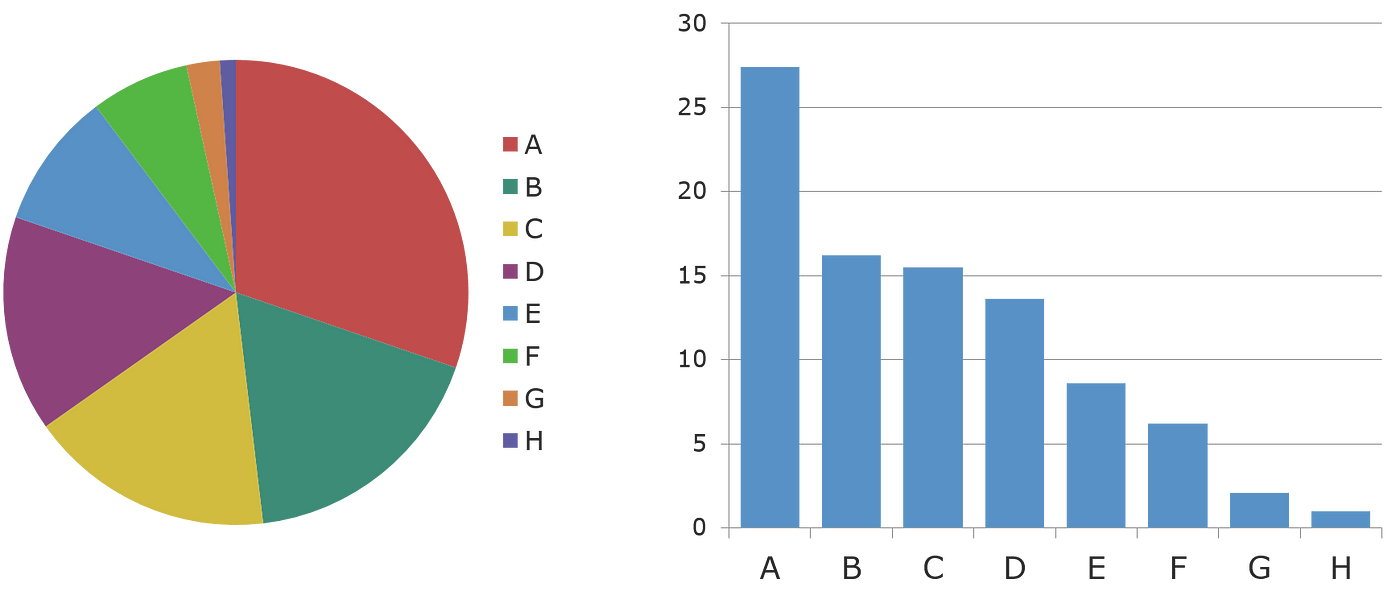
\includegraphics[width=\textwidth]{./imagem.png}
	\caption{Aqui é a legenda da imagem salva}\par
\end{figure}

E tabelas também podem ser flutuantes
\begin{table}
	\centering
	\begin{tabular}{|l|c|r|}
		\hline
		foo   & bar    & fubar \\
		fubar & toobar & foo   \\
		\hline
	\end{tabular}
	\caption{Legenda da tabela}
\end{table}

\end{document}
